%--------------------------------------
% Spécifications du chat Felix - Camix
%
% Domaine
%--------------------------------------

\section{Domaine}
\label{sec:domaine}

Un chat est muni de canaux pouvant accueillir des utilisateurs (cf. figure~\ref{sec:domaine:figchat}). Les utilisateurs peuvent communiquer entre eux au sein d'un même canal. Un utilisateur est reconnu par les autres utilisateurs par son surnom. Le surnom par défaut est un point d'interrogation (\texttt{?}). Un canal est identifié par son nom.

\medskip
\begin{figure}[h!]
\begin{center}
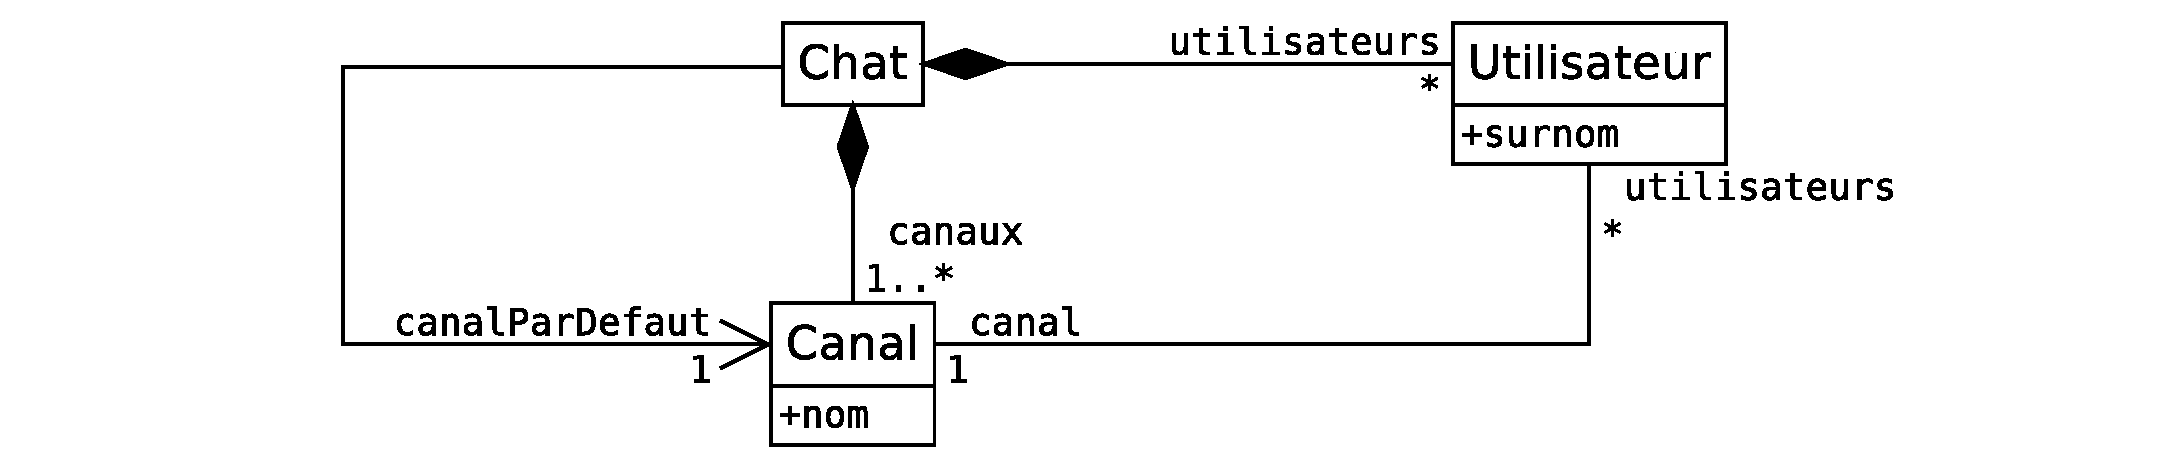
\includegraphics[width=\linewidth]{../img/Chat_Domaine.eps}
\caption{Diagramme de classes du domaine du chat.}
\label{sec:domaine:figchat}
\end{center}
\end{figure}

